\chapter{引言}
\label{cha:intro}

\section{研究背景}
\label{sec:background}
互联网的出现使人与人之间的交流变得简单轻松,信息交流更加便捷,各种各样的网络服务层出不穷,共享单车、网约车和在线教育就在很短的时间内让人们的生活发生了很大的改变。人们都频繁在网上获取信息,并寻找更加优质的服务。因此,它很大程度上改变了人们的生活方式,让人们的生活变得丰富多彩。第41次《中国互联网络发展状况统计报告》\cite{networkreport}指出,截至 2018年6月,我国网民规模已达到了8.02亿,半年之内我国新增2968万网民,每天平均几乎有16万新网民加入互联网,我国的互联网已经成为很多人必不可少的一部分。不仅仅是人们生活实用互联网频率不断增加,很多企业也使用互联网管理设备和存储用户信息。

在这种情况下,网络安全问题就会对我们的社会造成极大的损失。有很多网络非法行为给人们造成了很多损失。2018年8月3日,台积电(TSMC)被病毒Wannacry病毒入侵,它的基地生产线摆停。虽然最后病毒被成功清理,但是台积电也因此预计造成约17.6亿元人民币损失。同年8月28日,华住酒店信息泄露,其中涉及姓名、身份证号、邮箱、家庭住址、开房记录等敏感信息约5亿条被出售。

我们需要重视网络安全问题,网络安全问题很可能会让我们蒙受不必要的损失。在众多网络安全攻击中,拒绝服务攻击(Denial of Service, DoS)攻击作为一种普遍而又威力强大的攻击,被黑客广泛的使用,对互联网的系统造成了极大的危害。而分布式拒绝服务攻击(Distributed Denail of Service, DDoS)作为DoS攻击的新模式,它拥有更加强大的攻击威力和更好的隐蔽性,使无数的企业都为该类攻击所困扰。


2018年1月29日, DDoS攻击迫使荷兰三大银行(荷兰银行、荷兰合作银行和ING银行)的服务器超载。因此,它们网站和互联网银行服务瘫痪,荷兰税务局也遭受到类似的处境。
% http://www.sohu.com/a/272186665_100238920

2018年2月28日,世界上最顶尖的代码托管网站Github遭受了DDoS攻击并因此在几分钟内无法提供正常的服务,使很多公司都收到了影响。该攻击的峰值速率高达1.35Tb/s,超过了以往的所有DDoS峰值速率记录记录。
% http://www.sohu.com/a/272186665_100238920

2018年4月17日,美国的网络安全服务运营商Sucuri也遭受了大规模的DDoS攻击,导致一些端口的吞吐量达到容量上限,因此有非常高的延迟甚至还出现了数据包的丢失。因此,在西欧、南美和美国东部部分地区的服务被迫中断。
% http://www.cert.org.cn/publish/main/98/2018/20180426085352471430574/20180426085352471430574_.html

2018年5月13日,丹麦的铁路运营商(DSB)的系统受到了DDoS攻击,该公司的售票机、商店还有旅客的手机客户端都无法完成购票流程。因此,该公司不得不采用人工售票的方式暂时缓解压力,直到5月14日上午才能得到解决。这次事件让1.5万旅客受到了影响。
%http://www.cert.org.cn/publish/main/98/2018/20180518143816118933026/20180518143816118933026_.html

在卡巴斯基实验室2018年第四季度的调查中,我国的网络安全形势依然不容更乐观,中国依然是全世界范围内受DDoS最严重的国家,所以,我们需要重视DDoS的防御问题。
% https://securelist.com/ddos-attacks-in-q4-2018/89565/

\begin{figure}
    \centering
    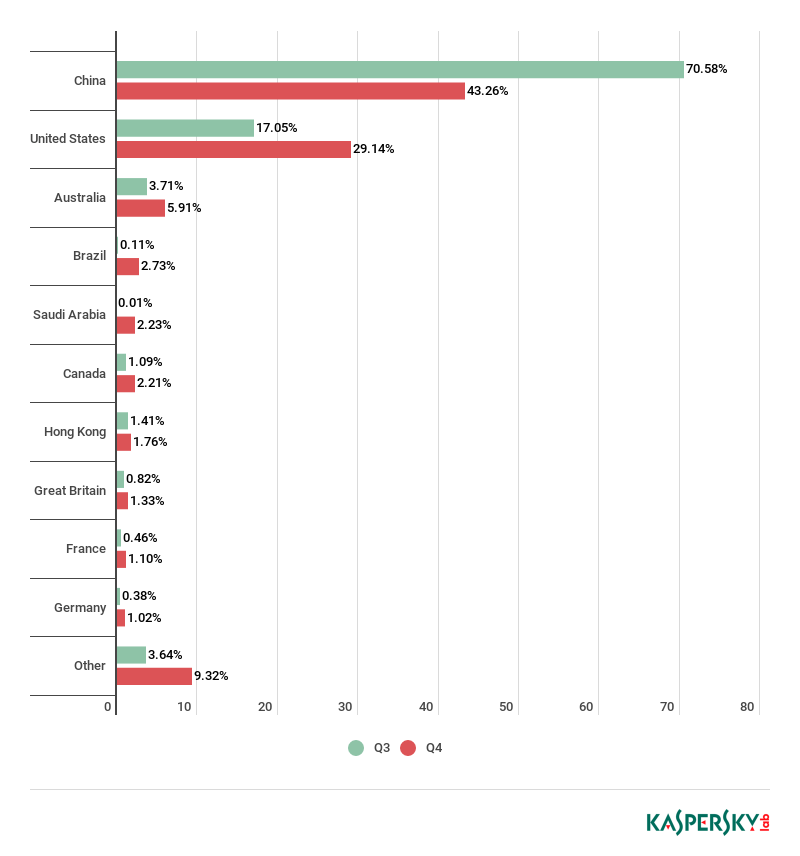
\includegraphics[scale=0.5]{figures/en-ddos-by-countries.png}
    \caption{在2018年Q3和Q4中,世界各国受DDoS攻击分布}
    \label{fig:ddos_countries}
\end{figure}

DoS攻击的危害是很大的,而且它的实现形式也是各不相同。在所有的DoS攻击种类中,低速率服务拒绝(Low-rate Denial of Service,LDoS)攻击\cite{LDoS}是一种针对良性TCP流最有效的一种攻击。和直接发送大量流量的洪泛方式不同,它通过发送周期性的脉冲低速流就可以持续迫使TCP流进入超时重传的等待阶段,造成TCP流吞吐量显著下降的可怕后果。而且由于LDoS攻击的并非洪泛的方式,平均速率很低。相对于洪泛方式的DoS攻击,LDoS攻击更加难以被检测,而且,LDoS攻击以分布式方式实现的时候,LDoS攻击的隐蔽性更加强。
% Among all kinds of DoS attacks, the low-rate TCP attack~\cite{b20} is essentially the most efficient in terms of causing damage to benign TCP flows. Instead of directly sending a huge amount of traffic, it generates periodically pulsing low-rate flows to cause continuous retransmission of benign TCP flows, which results in significant throughput degradation. Due to the low rate, such attack is more difficult to be detected compared to flooding-based attacks. Moreover, the attack can be launched in a distributed mode, which further increases its stealthiness.
目前,为了有效的防御LDoS攻击,

\section{主要研究内容}
\label{sec:work}

\section{主要贡献}
\label{sec:contribution}

\section{文章内容安排}
\label{sec:contribution}

